\chapter{示例}
\label{chp:example}
本部分为列表、表格、图片等示例
\section{列表示例}
\begin{itemize}[leftmargin=*]
	\item 这是一个列表项目
	\item 这是一个列表项目
	\item 这是一个列表项目
	\item 这是一个列表项目
	\item 这是一个列表项目
\end{itemize}
\section{引用示例}
\label{sec:ref}
文档的各个部分引用前均需采用 \textbackslash label 命令添加标签,图表公式添加在环境内部,所需引用章节添加于命令之后,建议对不同类型label 命名时进行区分。

参考文献引用:\cite{liu_approaching_2018},图片引用:如图 \ref{picexam}所示,表格引用:如表\ref{tbl:pre_processing}所示,公式引用:如式(\ref{eq:111})所示,章节引用:第 \ref{chp:example}章、第  \ref{sec:ref}节、第 \ref{ssec:pic}节。

\section{图片}
论文中的图片插入通常在一下方式中选择一种即可,每次插入可以拷贝一份粘贴至目标位置,并更改路径、大小、标题和label。
\subsection{无子图图片}
通常来说,论文中的图片插入时只有一个文件,子图应在外部拼接好后导出为一整张图片,再进行导入,并且由于材料学院双语标题要求,采用\textbackslash bicaption{中文}{英文}实现,前者为中文,后者为英文。如不需要双语标题,改为\textbackslash caption{标题}即可。
\label{ssec:pic}
\begin{figure}[H]
	\centering
	
\includegraphics[width=0.6\textwidth]{figure/chapter1/Omni.jpg}%设置图片宽度和源文件路径,无命名冲突时可不包含文件类型后缀
	\bicaption{不带子图图片示例,(a)1,(b)2,(c)3,(d)4}{This is an english title}% 双语标题
	\label{picexam}%标签
\end{figure}

\begin{figure}[H]
	\centering
	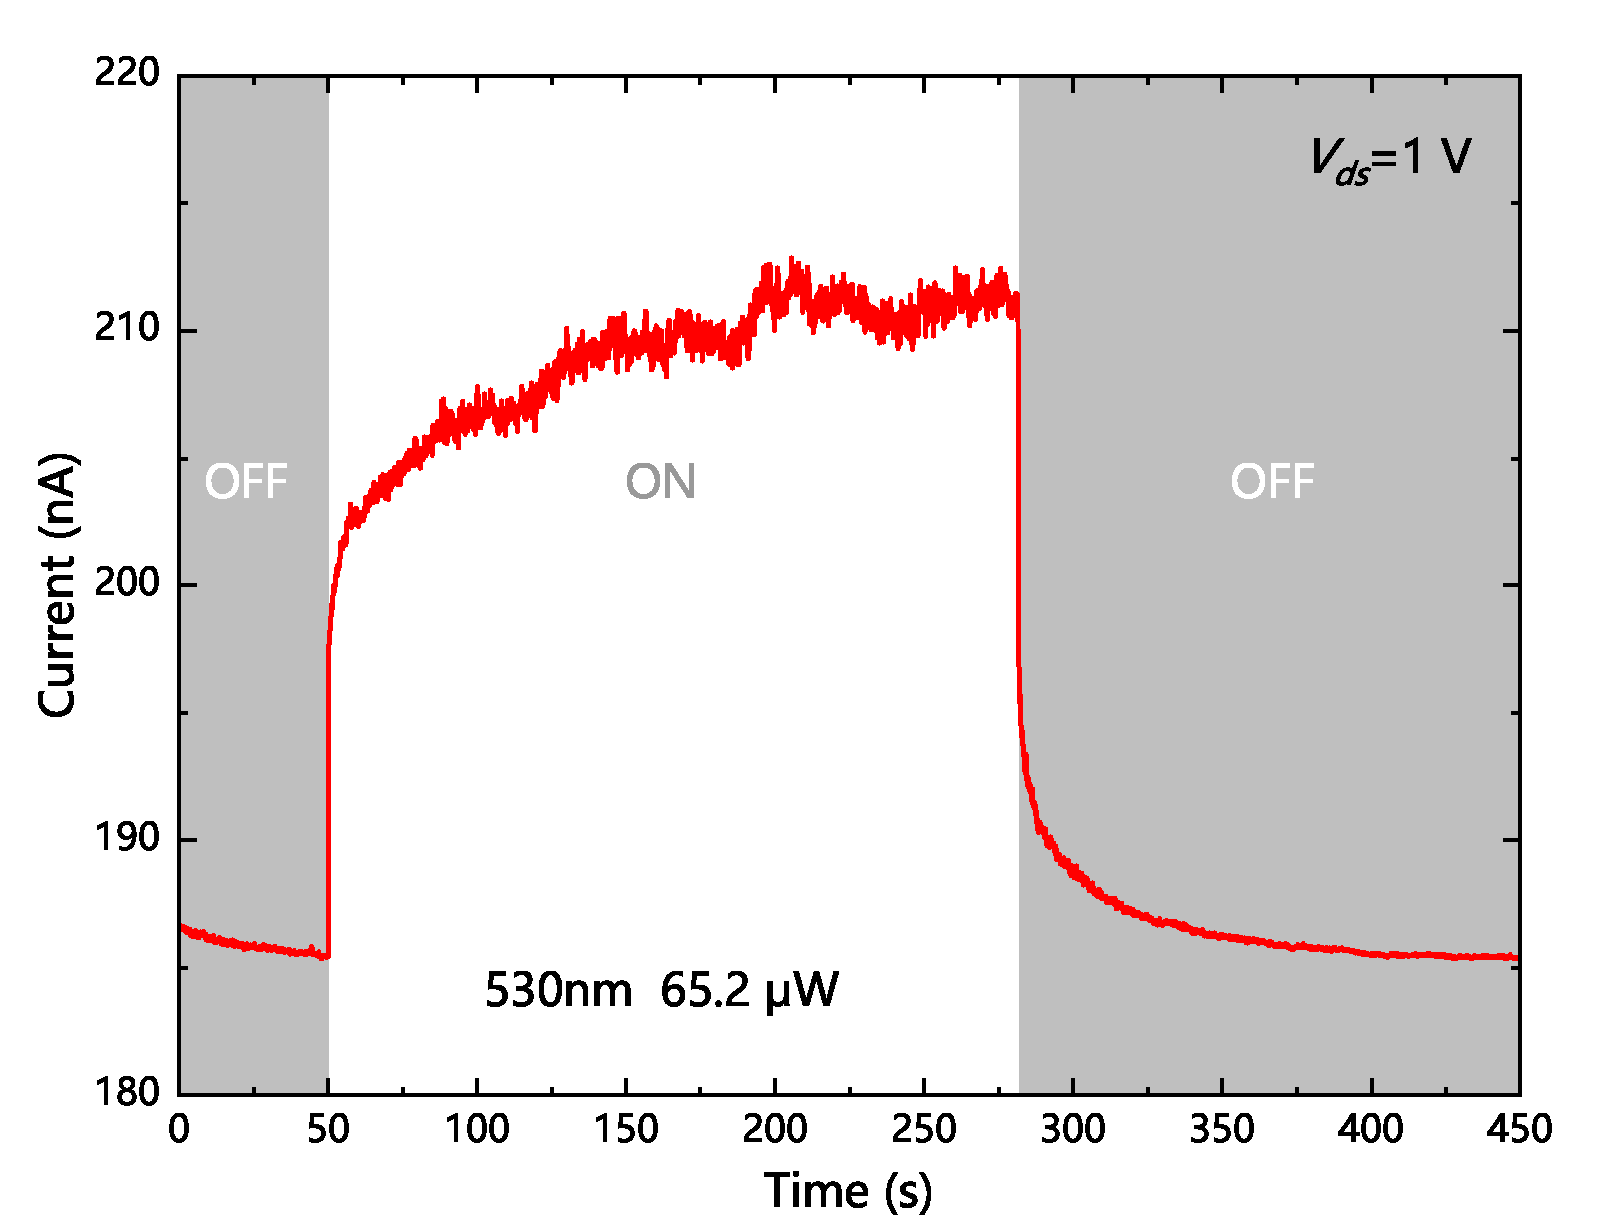
\includegraphics[width=0.6\textwidth]{figure/chapter1/Graph3.pdf}
	\caption{矢量图片示例,无英文标题}	
	\label{pdfpic}
\end{figure}
\subsection{带有子图图片}
如坚持使用子图插入的类型,可以采用如下格式:
\begin{figure}[H]
	\centering
	\subfigure[]{
		
\includegraphics[width=0.21\textwidth]{figure/chapter1/Omni.jpg}}
	\subfigure[]{
		
\includegraphics[width=0.21\textwidth]{figure/chapter1/Omni.jpg}}\\%分行
	\subfigure[]{
		
\includegraphics[width=0.21\textwidth]{figure/chapter1/Omni.jpg}}
	\hspace{3cm}
	\subfigure[]{
		
\includegraphics[width=0.21\textwidth]{figure/chapter1/Omni.jpg}}
	
	\bicaption{带子图图片示例,(a)1,(b)2,(c)3,(d)4}{This is an english figure title}
	\label{fig:binaural_recording}
\end{figure}

视频提供了功能强大的方法帮助您证明您的观点。当您单击联机视频时,可以在想要添加的视频的嵌入代码中进行粘贴。您也可以键入一个关键字以联机搜索最适合您的文档的视频。
为使您的文档具有专业外观,Word 提供了页眉、页脚、封面和文本框设计,这些设计可互为补充。例如,您可以添加匹配的封面、页眉和提要栏。单击“插入”,然后从不同库中选择所需元素。
主题和样式也有助于文档保持协调。当您单击设计并选择新的主题时,图片、图表或 SmartArt 图形将会更改以匹配新的主题。当应用样式时,您的标题会进行更改以匹配新的主题。

\section{表格}
表格与图片类似,但表格和图片独立编号,且标题在上。一般来说论文中应采用三线表,但为了应对特殊需求,以下仍给出普通表格示例:
\subsection{普通表格}
\begin{table}[H]
	\caption{HRTF 预处理方法}
	\centering
	\begin{tabular}{|c|c|c|}
		\hline
		方法 & 预处理对象 & 预处理方法 \\
		\hline
		$H_{a}$ & 复频谱 & 时间对准 \\
		$H_{s m}$ & \multicolumn{1}{l|}{复频谱} & 平滑 \\
		$|H|$ & 幅度谱 & 无 \\
		
		\hline
	\end{tabular}
\end{table}

\subsection{三线表}
三线表示例如下,\textbackslash toprule 和 \textbackslash bottomrule为粗线,\textbackslash midrule为细线,toprule和midrule之间应为表格标题行。
\begin{table}[H]
	\bicaption{HRTF 预处理方法}{ HRTF pre-process mothod}
	\centering
	\begin{tabular*}{\hsize}{@{\extracolsep{\fill}}ccc}
		\toprule
		方法 & 预处理对象 & 预处理方法 \\
		\midrule
		$H_{a}$ & 复频谱 & 时间对准 \\
		$H_{s m}$ & 复频谱 & 平滑 \\
		$|H|$ & 幅度谱 & 无 \\
		\bottomrule
	\end{tabular*}
	\label{tbl:pre_processing}
\end{table}



\begin{table}[htbp]
	\centering
	\caption{Comparison of different obfuscations in terms of their transformation capabilities}
	\begin{tabular}{ccccc} % 控制表格的格式
		\toprule
		\multirow{2}{*}{Obfuscators} & \multicolumn{4}{c}{Transformations}   \\
		\cline{2-5}  % 这部分是画一条横线在2-6 排之间
		&    Renaming & Dead code removal & control flow obfuscation & string encryption \\
		\midrule
		Proguard &  \checkmark & $\times$  & $\times$ & \checkmark   \\
		Allatori & \checkmark & $\times$  & $\times$ & \checkmark \\
		DashO & \checkmark & $\times$  & $\times$ & \checkmark \\
		Androcrypt & \checkmark & $\times$  & $\times$ & \checkmark  \\
		\bottomrule
	\end{tabular}
	\label{tbl:table1}
\end{table}

\section{公式}
公式示例如下:

不带编号公式:
\[
M=
\left[
\begin{matrix}
	\textcolor{red}{\varepsilon_{11}} & \varepsilon_{12} & \varepsilon_{13}\\
	\varepsilon_{21} & \varepsilon_{22} & \varepsilon_{23}\\
	\varepsilon_{31} & \varepsilon_{32} & \varepsilon_{33}\\
\end{matrix}\right]
\]
\[
\mu = \frac{B}{H}=\frac{B_0 e^{i\omega t-\delta}}{H_0 e^{i\omega t}}=\frac{B_0}{H_0}\cos\delta-i\frac{B_0}{H_0}\sin\delta
\]

带编号公式:
\begin{equation}
	\eta = \frac{qVN_0}{d^2}\left\{(\mu\tau)_e \left[1-\text{exp}\left(\frac{x_0-d}{\frac{(\mu\tau)_e V}{d}}\right)\right]+(\mu\tau)_h \left[1-\text{exp}\left(\frac{-x_0}{\frac{(\mu\tau)_h V}{d}}\right)\right]\right\}
\end{equation}

多行带编号公式:
\begin{align}
	\label{eq:111}
	\phi & = \text{mod}~\left( 360^{\circ}-\varphi_{\text{SOFA}}, 360^{\circ} \right)  \nonumber \\
	\theta & =  90^{\circ} - \theta_{\text{SOFA}} 	
\end{align}


